%---------------------------------------------------------------------------------------------------------------------------------------------
%                                                            HEADER
%---------------------------------------------------------------------------------------------------------------------------------------------
% ¿Qué secciones debe contener una presentación?

% Índice
% Introducción al tema
% Desarrollo del proyecto
% Conclusiones 
% Trabajo Futuro
% Invitación a preguntas
% Agradecimiento y despedida
 
% ¿Aproximadamente cuántas filminas?

% Lo ideal es que la presentación ronde los 30min (y no exceda los 40min). Si en promedio dedicamos 3min por filmina, 10 a 12 filminas útiles es un número razonable. Con "útiles" me refiero a las de contenido, no separadores ni indicativas.

% Recuerden que lo importante es lo que uds. hicieron. El marco teórico está en el informe y con 1 o 2 filminas debería ser suficiente.

% INSERTAR FIGURAS EJEMPLO
%\begin{figure}[ht]
%    \centering
%    \vspace{-0.50cm}
%    \scalebox{0.25}{\includegraphics[angle=0]{./oh_source.eps}}
%\end{figure}

\documentclass{beamer}
\graphicspath{{./figuras/}}
\mode<presentation>
{
    \usebackgroundtemplate{
\includegraphics[width=\paperwidth]{fondo_2.jpg}}
    \usetheme{default}      % or try Darmstadt, Madrid, Warsaw, default...
    \usecolortheme{default} % or try albatross, beaver, crane, default ...
    \usefonttheme{default}  % or try serif, structurebold, ...
    \setbeamertemplate{navigation symbols}{}
    \setbeamertemplate{caption}[numbered]
} 

\usepackage[english]{babel}
\usepackage[utf8x]{inputenc}

\title[Your Short Title]{Infraestructura tecnológica virtual con automatización y orquestación.}
\author{Arese, Juan Pablo - Diers, Werner Christian}
\institute{Facultad de Ciencias Exactas, Físicas y Naturales - UNC}
\date{Febrero 2017}

\begin{document}


%---------------------------------------------------------------------------------------------------------------------------------------------
%                                                                TITULO
%---------------------------------------------------------------------------------------------------------------------------------------------
\begin{frame}
  \titlepage
\end{frame}


%---------------------------------------------------------------------------------------------------------------------------------------------
%                                                   ORGANIZACIÓN DE LA PRESENTACIÓN
%---------------------------------------------------------------------------------------------------------------------------------------------
\section{Organización de la Presentación}

\begin{frame}{Organización de la Presentación}
    \vspace{-1.5cm}
    La precentación esta organizada de manera incremental explicando cada uno de los siguientes puntos.\\
    \begin{itemize}
        \item Introduccion.
        \item Objetivos.
        \item Arquitectura.
        \item Desarrollo del sistema.
        \begin{itemize}
            \item Herramienta de virtualizacion.
            \item Herramienta de aprovicionamiento.
            \item Herramienta de orquestacion.
            \item Interfaz web.
        \end{itemize}
    \end{itemize}

\end{frame}


%---------------------------------------------------------------------------------------------------------------------------------------------
%                                                             INTRODUCCION
%---------------------------------------------------------------------------------------------------------------------------------------------
\section{Introduccion}

\begin{frame}
    %\vspace{}
    \Huge
    \centering
    \textbf{ Introduccion }

\end{frame}


\begin{frame}{Introduccion}
    \vspace{-1.5cm}
    La cantidad de servicios y servidores necesarios en las organizaciones tiende a ser cada vez mayor.
    Cada día los despliegues son más complejos, siendo necesario trabajar con aplicaciones clusterizadas, múltiples datacenters,etc.
    Este tipo de tareas ya no pueden realizarse individualmente para cada máquina y menos aún en entornos escalables donde pueden haber cientos de nodos.

    \begin{block}{}
        Hablar de orquestación implica eficiencia en los recursos, tanto humanos como computacionales, y por ello implica hablar de virtualización, provisionamiento y datacenters dinámicos. En este sentido, virtualización puede aplicar a computadoras, sistemas opera
        tivos, dispositivos de almacenamiento, aplicaciones o redes.
    \end{block}

\end{frame}

\begin{frame}{Introduccion}
    \vspace{-1.5cm}
    \textbf{¿Qué es virtualización?}

    Virtualización es un término para software ejecutándose, usualmente sistemas operativos, de manera concurrente y aislada de otros programas en el mismo sistema. 

    \begin{block}{}
        Muchas de las implementaciones de virtualización utilizan un hypervisor, una capa de software que controla el hardware y provee sistemas operativos huéspedes con acceso a los dispositivos de hardware subyacentes. 
    \end{block}

    \begin{block}{}
        El hypervisor permite ejecutar múltiples sistemas operativos en el mismo sistema físico ofreciendo hardware virtualizado al sistema operativo huésped.
    \end{block}

\end{frame}

\begin{frame}{Introduccion}
    \vspace{-1.5cm}
    \textbf{¿Qué es aprovisionamiento?}

    En general, aprovisionamiento, significa proveer o hacer que algo esté disponible. El término es utilizado en un gran variedad de contextos en el área de Tecnologías de Información. En este Proyecto Integrador, el término hace referencia a lo siguiente:

    \begin{block}{}
    \textit
    {
        Aprovisionamiento es el conjunto de acciones para preparar una máquina virtual, con el sistema apropiado, datos y software, y dejarla lista para su operación.
    }
    \end{block}

\end{frame}

\begin{frame}{Introduccion}
    \vspace{-1.5cm}
    \textbf{¿Qué es orquestación?}

    La orquestación es automatizar procesos y flujos de trabajo mientras que la automatización básicamente automatiza una tarea específica.
    Un orquestador es una pieza de software (middleware) que permite integrar servicios provenientes de diversas fuentes, y proveer información de forma síncrona o asíncrona, a través del uso de servicios web, bases de datos, archivos, entre otras fuentes y destinos.

\end{frame}
%---------------------------------------------------------------------------------------------------------------------------------------------
%                                                           OBJETIVOS
%---------------------------------------------------------------------------------------------------------------------------------------------
\section{Objetivos}

\begin{frame}
    %\vspace{}
    \Huge
    \centering
    \textbf{ Objetivos }

\end{frame}

\begin{frame}{Objetivo principal}
    \vspace{-1.5cm}
    Un sistema de infraestructura virtual automatizado y con orquestación tiene como objetivo brindar a los administradores de servidores una herramienta que facilite la preparación y configuración de sus sistemas de manera simple.

    \begin{block}{}
        El objetivo principal de este proyecto es integrar diferentes herramientas con el fin de implementar técnicas de orquestación, virtualización, instalación y configuración automática para facilitar la gestión de servidores virtuales y sus servicios asociados.
    \end{block}

\end{frame}


\begin{frame}{Objetivos secundarios}
\vspace{-1.5cm}
\begin{itemize}
    \item Instalar y utilizar sistemas operativos para servidor.
    \item Emplear herramientas de virtualización.
    \item Usar herramientas de aprovisionamiento.
    \item Utilizar herramientas de orquestación.
    \item Analizar protocolos para booteo a través de la red.
\end{itemize}

\end{frame}


%---------------------------------------------------------------------------------------------------------------------------------------------
%                                                            ARQUITECTURA
%---------------------------------------------------------------------------------------------------------------------------------------------
\section{Arquitectura}

\begin{frame}
    %\vspace{}
    \Huge
    \centering
    \textbf{ Arquitectura }

\end{frame}

\begin{frame}{Arquitectura}
    \vspace{-1.5cm}
    La arquitectura implementada es la de Cliente-Servidor.
    Las tareas del servidor son las siguientes:
    \begin{itemize}
        \item Crear las maquinas virtuales.
        \item Asignar direcciones IP via servidor DHCP.
        \item Aprovicionar la maquina con el SO deseado y los parametros de configuracion establecidos.
        \item Orquestar las politicas definidas para una maquina o un conjunto de maquinas.
    \end{itemize}

\end{frame}

\begin{frame}{Arquitectura}
    \vspace{-1.5cm}
    \begin{figure}[ht]
       \centering
       \vspace{-0.50cm}
       \scalebox{0.35}{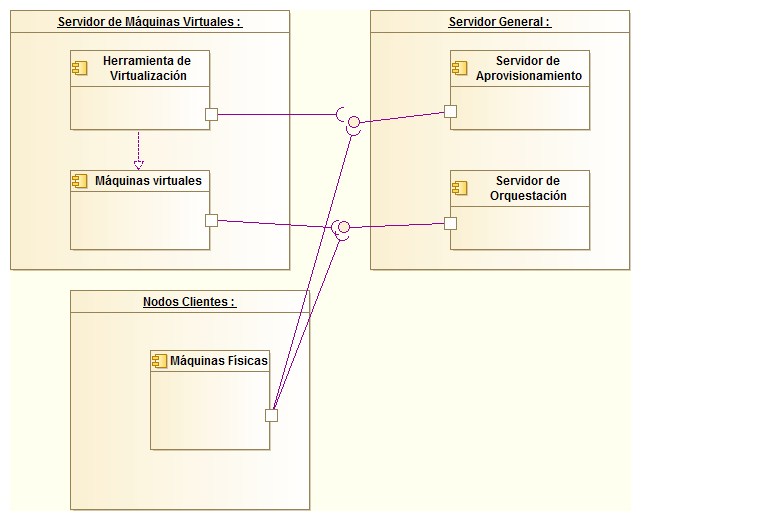
\includegraphics[angle=0]{./figuras/ArquitecturaDeDesarrolloEnUnEntornoMixto.png}}
    \end{figure}

\end{frame}


%---------------------------------------------------------------------------------------------------------------------------------------------
%                                                                DESARROLLO
%---------------------------------------------------------------------------------------------------------------------------------------------
\section{Desarrollo}
\begin{frame}
    %\vspace{}
    \Huge
    \centering
    \textbf{ Desarrollo }

\end{frame}

\begin{frame}{Desarrollo - Virtualizacion}
    \vspace{-1.5cm}
    La herramienta utilizada para virtualizar fue KVM/Qemu.

    KVM utiliza virtualización completa:
    \begin{itemize}
        \item Es una forma virtualización donde el sistema operativo huésped desconoce que está en un entorno virtual.
        \item El hardware se encuentra virtualizado por el sistema operativo anfitrión. 
        \item La capa de virtualización, un hypervisor, media entre los sistemas huéspedes y el anfitrión. 
    \end{itemize}

\end{frame}

\begin{frame}{Desarrollo - Virtualizacion}
    \vspace{-1.5cm}
    \begin{figure}[ht]
       \centering
       \vspace{-0.50cm}
       \scalebox{0.60}{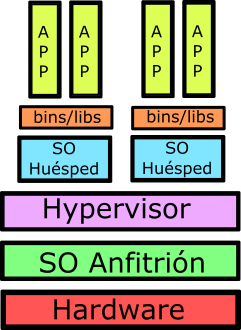
\includegraphics[angle=0]{./figuras/virtualizacion_tipos_3.png}}
       %+INSERTAR ACA LA IMAGEN DE VIRTUALIZACION COMPLETA\\
    \end{figure}

\end{frame}

\begin{frame}{Desarrollo - Virtualizacion}
    \vspace{-1.5cm}
    \begin{figure}[ht]
       \centering
       \vspace{-0.50cm}
       \scalebox{0.25}{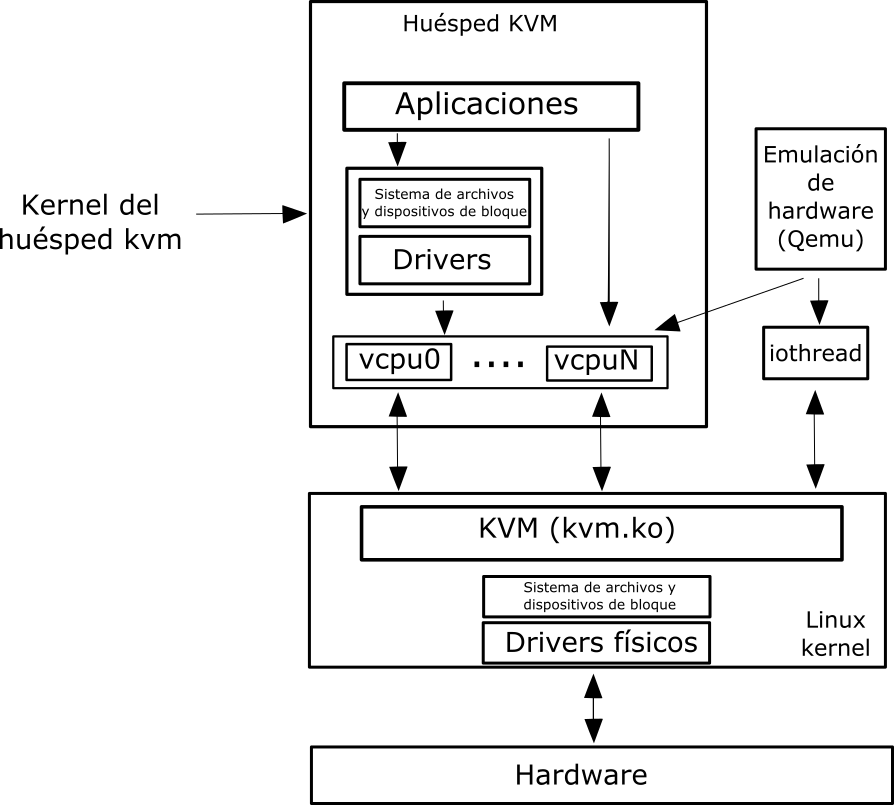
\includegraphics[angle=0]{./figuras/kvm_arquitectura_1.png}}
       %+INSERTAR ACA LA IMAGEN DE LA ARQUITECTURA DE LA VIRTUALIZACION DE KVM
    \end{figure}

\end{frame}

\begin{frame}{Desarrollo - Aprovisionamiento}
    \vspace{-1.5cm}
    La herramienta utilizada para el aprovisionamiento fue Cobbler.
    \begin{block}{}
        Es un servidor del aprovisionamiento Linux que centraliza y simplifica el control de servicios incluyendo PXE, DHCP, TFTP, y DNS con propósito de realizar instalaciones basadas en red de sistemas operativos.
    \end{block}

    \begin{block}{}
        Cobbler utiliza objetos para definir la configuración de aprovisionamiento:
    \end{block}

\end{frame}

\begin{frame}{Desarrollo - Aprovisionamiento}
    \vspace{-1.5cm}
    \begin{figure}[ht]
       \centering
       \vspace{-0.50cm}
       %\scalebox{0.25}{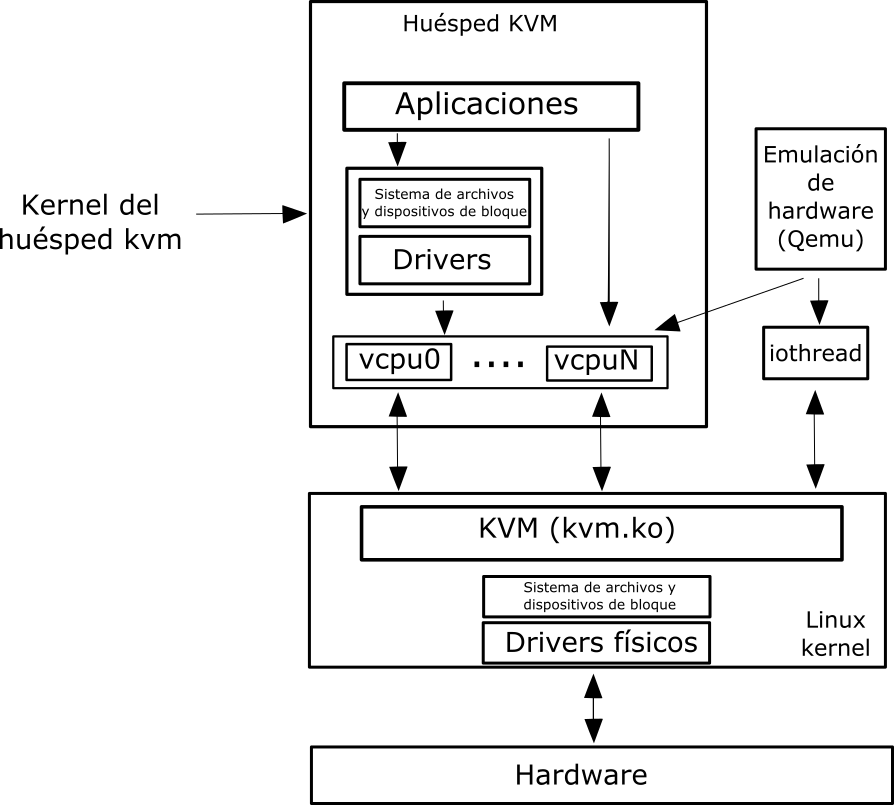
\includegraphics[angle=0]{./figuras/kvm_arquitectura_1.png}}
       %+INSERTAR ACA LA IMAGEN DE LA ARQUITECTURA DE MODELADO DE COBBLER
    \end{figure}
\end{frame}

\begin{frame}{Desarrollo - Aprovisionamiento}
    \vspace{-1.5cm}
    \begin{itemize}
        \item Distro: Distribución que se desea instalar. 
        \item Repo: Un repositorio, sitio centralizado donde se almacena y mantiene información digital.
        \item Perfil: Asocia una distribución a opciones especializadas adicionales, como puede ser un archivo de configuración.
        \item Imágen: Copia del estado de un sistema computacional, guardado en un archivo o disco.
        \item Sistema: Mapea una pieza de hardware (o una máquina virtual) con el perfil asignado a correr en ella. 
    \end{itemize}

\end{frame}

\begin{frame}{Desarrollo - Aprovisionamiento}
    \vspace{-1.5cm}
    \begin{figure}[ht]
       \centering
       \vspace{-0.50cm}
       %\scalebox{0.25}{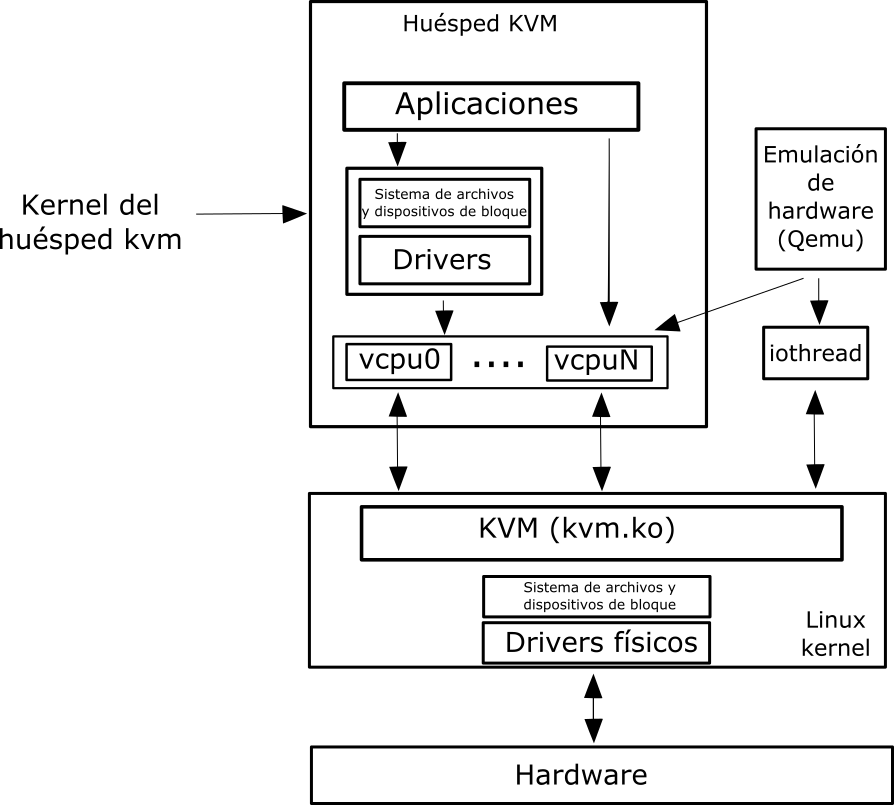
\includegraphics[angle=0]{./figuras/kvm_arquitectura_1.png}}
       %+INSERTAR ACA LA IMAGEN DE LA INTERFAZ WEB DE COBBLER MOSTRANDO PERFILES, SISTEMAS; DISTROS, ETC CREADOS
    \end{figure}

\end{frame}

\begin{frame}{Desarrollo - Aprovisionamiento}
    \vspace{-1.5cm}
    \begin{figure}[ht]
       \centering
       \vspace{-0.50cm}
       %\scalebox{0.25}{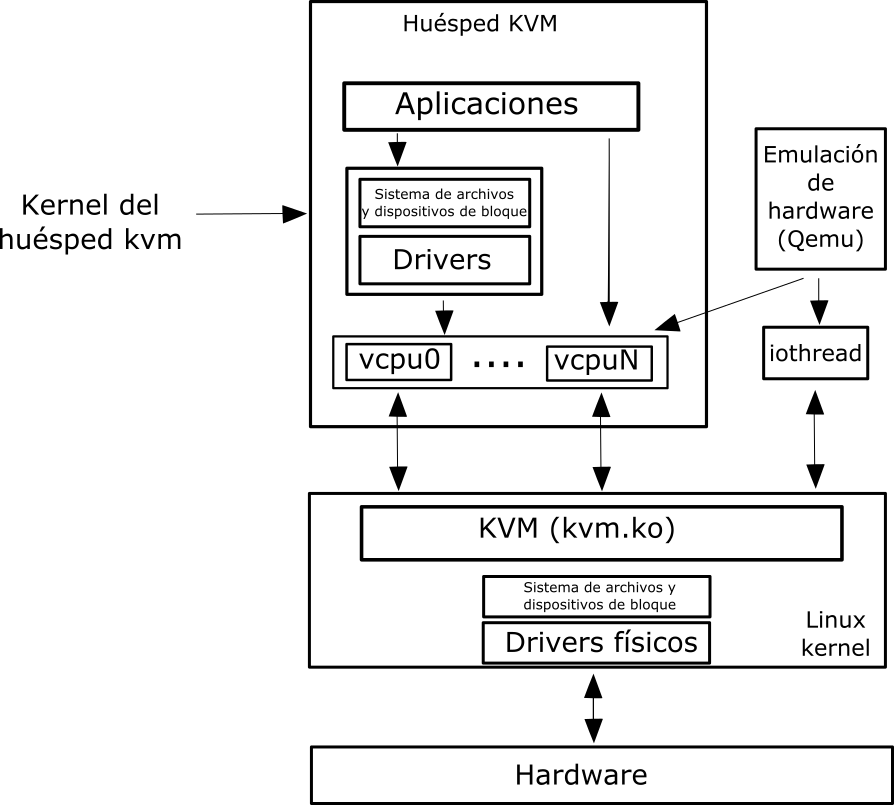
\includegraphics[angle=0]{./figuras/kvm_arquitectura_1.png}}
       %+INSERTAR ACA LA IMAGEN DE LA INTERFAZ WEB DE COBBLER MOSTRANDO PERFILES, SISTEMAS; DISTROS, ETC CREADOS
    \end{figure}

\end{frame}

\begin{frame}{Desarrollo - Orquestación}
    \vspace{-1.5cm}
    La herramienta utilizada para orquestar fue Puppet.

    Utiliza una arquitectura cliente/servidor.  
    \begin{itemize}
        \item El servidor necesariamente debe correr en un sistema basado en Unix.
        \item El usuario describe los recursos del sistema y sus estados utilizando un lenguaje declarativo.    
        \item El nodo maestro (servidor) provee una interfaz HTTPS con varios extremos disponibles.
        \item Cuando se pide o envía cualquier dato al servidor, el agente hace un pedido HTTPS o a uno de esos extremos. 
    \end{itemize}

\end{frame}


\begin{frame}{Desarrollo - Orquestación}
    \vspace{-1.5cm}
        \begin{figure}[ht]
           \centering
           \vspace{-0.50cm}
           \scalebox{0.25}{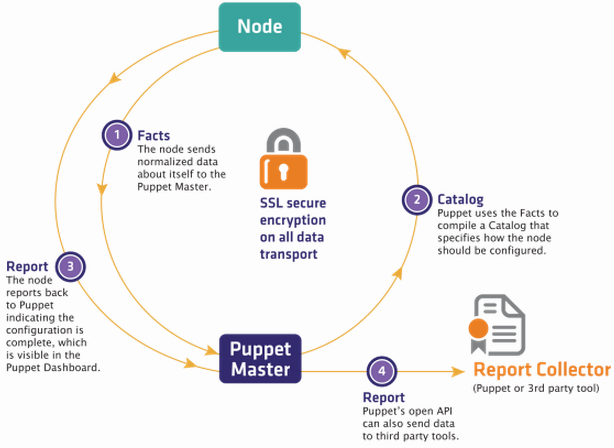
\includegraphics[angle=0]{./figuras/PuppetLabsEnforceDesiredState.png}}
           %++INSERTAR ACA LA IMAGEN DE FUNCIONAMIENTO DE PUPPET\\
        \end{figure}

\end{frame}

\begin{frame}{Desarrollo - Orquestación}
    \vspace{-1.5cm}
    \begin{figure}[ht]
       \centering
       \vspace{-0.50cm}
       %\scalebox{0.25}{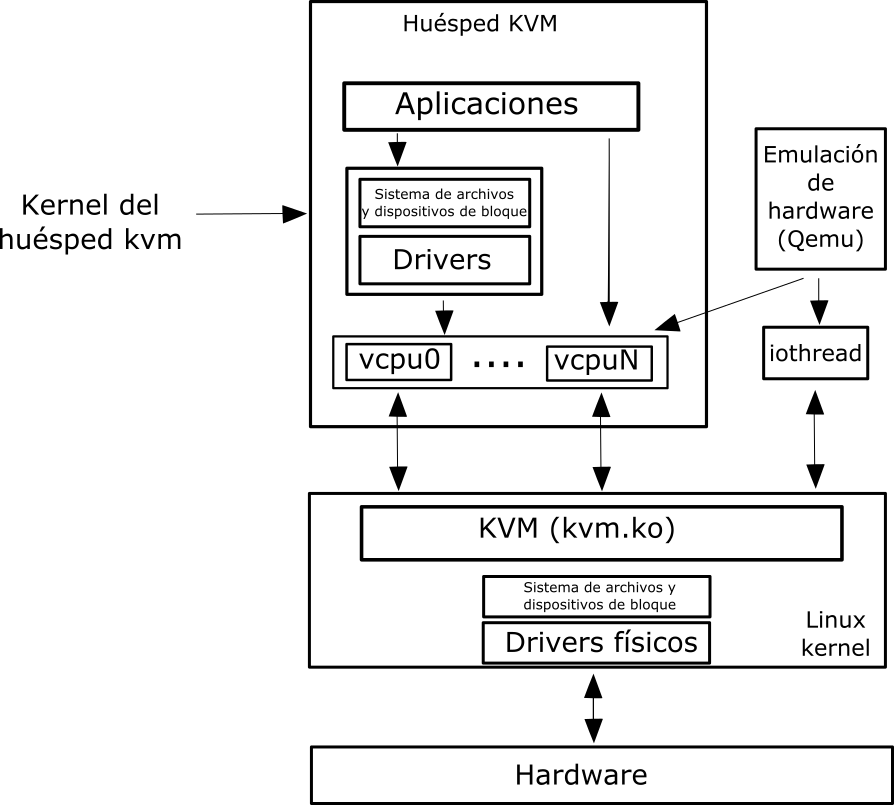
\includegraphics[angle=0]{./figuras/kvm_arquitectura_1.png}}
       %+INSERTAR ACA LA IMAGEN DE LA TERMINAL MOSTRANDO LOS NODOS ADMINISTRADOS\\
    \end{figure}

\end{frame}

\begin{frame}{Desarrollo - Orquestación}
    \vspace{-1.5cm}
    \begin{figure}[ht]
       \centering
       \vspace{-0.50cm}
       %\scalebox{0.25}{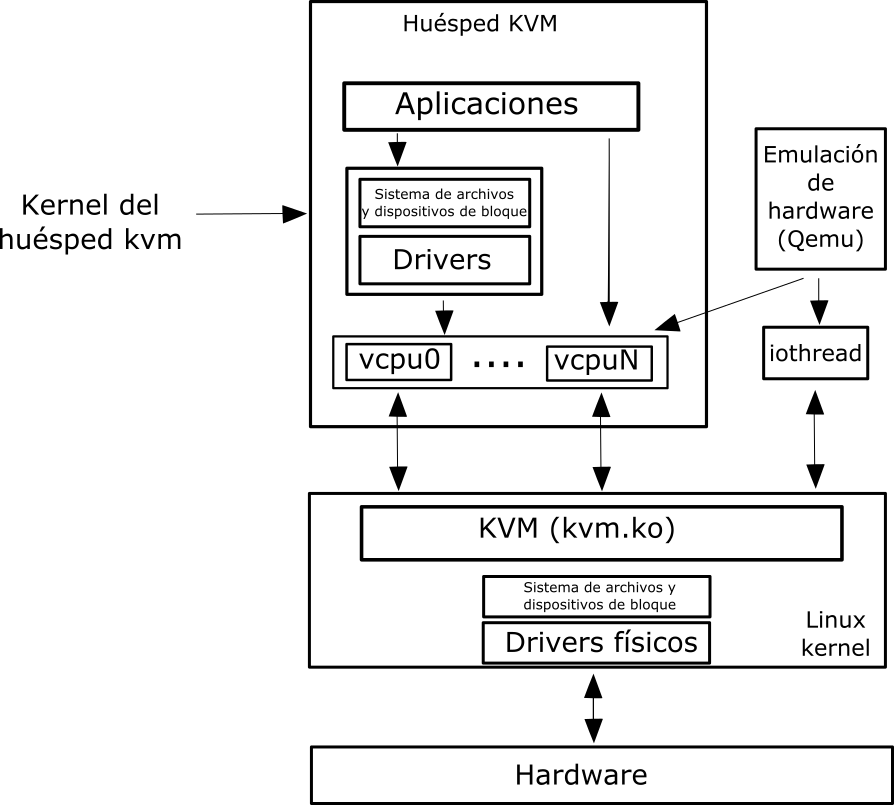
\includegraphics[angle=0]{./figuras/kvm_arquitectura_1.png}}
       %+INSERTAR ACA LA IMAGEN DE LA TERMINAL MOSTRANDO LA ESTRUCTURA DE MANIFIESTOS
    \end{figure}

\end{frame}

\begin{frame}{Desarrollo - Interfaz Web}
    \vspace{-1.5cm}
    La herramienta utilizada para crear la interfaz web fue Pyhton Bottle.

\end{frame}

\begin{frame}{Desarrollo - Interfaz Web}
    \vspace{-1.5cm}
    \begin{figure}[ht]
       \centering
       \vspace{-0.50cm}
       %\scalebox{0.25}{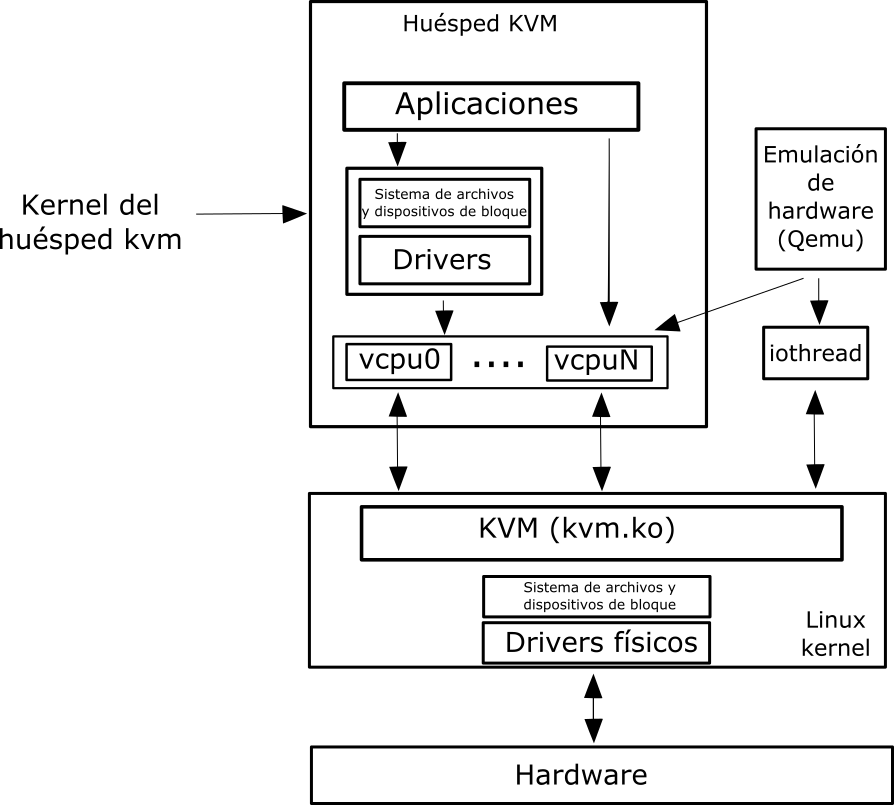
\includegraphics[angle=0]{./figuras/kvm_arquitectura_1.png}}
       %+INSERTAR ACA LA IMAGEN DE LA INTERFAZ WEB\\
    \end{figure}

\end{frame}

\begin{frame}{Desarrollo - Interfaz Web}
    \vspace{-1.5cm}
    \begin{figure}[ht]
       \centering
       \vspace{-0.50cm}
       %\scalebox{0.25}{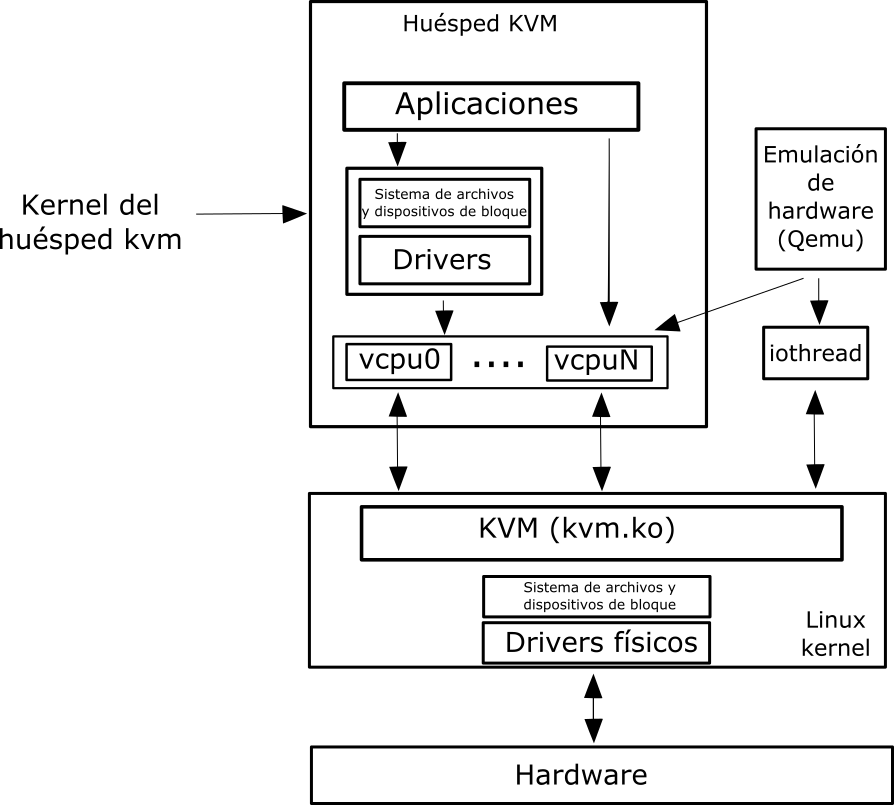
\includegraphics[angle=0]{./figuras/kvm_arquitectura_1.png}}
       %+INSERTAR ACA LA IMAGEN DE LA TERMINAL EJECUTANDO LA INTERFAZ WEB
    \end{figure}

\end{frame}
%---------------------------------------------------------------------------------------------------------------------------------------------
%                                                               CONCLUSIONES
%---------------------------------------------------------------------------------------------------------------------------------------------
\section{Conclusiones}
\begin{frame}
    %\vspace{}
    \Huge
    \centering
    \textbf{ Conclusiones }

\end{frame}

\begin{frame}{Conclusiones}
    \vspace{-1.5cm}
    El análisis formal del problema para la obtención de los requerimientos y los riesgos del proyecto, es algo que también debe destacarse. Esta es una fase imprescindible para poder llevar a cabo las estimaciones pertinentes a los tiempos de desarrollo e investigación de cualquier proyecto. En muchas ocasiones se cuenta con diferentes herramientas para llevar a cabo una misma tarea. El análisis de cada una de ellas y su elección, utilizando factores de decisión ponderados, es fundamental para el trabajo como ingeniero. De aquí también se puede hacer notar que la utilización de soluciones de código abierto no siempre permiten estar en la "cresta de la ola" tecnológica y muchas veces es necesario contar con software privativo para obtener la máxima producción.

\end{frame}


\begin{frame}{Conclusiones}
    \vspace{-1.5cm}
    El resultado final es positivo. El sistema final cumple con los requerimientos, es capaz de generar una gran cantidad de máquinas virtuales completamente equipadas y preparadas para desempeñar diferentes funciones, ya sean académicas o en entornos laborales, formando parte de una red nat con la cual cada maquina puede comunicarse con las demás maquinas de la red y tener acceso a internet.

\end{frame}


%---------------------------------------------------------------------------------------------------------------------------------------------
%                                                        TRABAJOS FUTUROS
%---------------------------------------------------------------------------------------------------------------------------------------------
\section{Trabajos Futuros}
\begin{frame}
    %\vspace{}
    \Huge
    \centering
    \textbf{Trabajos Futuros}

\end{frame}

\begin{frame}{Trabajos Futuros}
    \vspace{-1.5cm}
    \begin{itemize}
        \item Protección: Valoración de la probabilidad de que el sistema pueda resistir intrusiones accidentales o premeditadas. Para mejorar esta probabilidad se propone:
        \begin{itemize}
            \item  Modificar el sistema para que funcione con firewall y SELinux.

            \item  Incluir validación por usuario en la interfaz web. 

            \item  Incluir un log de cambios al sistema que permita saber quién y qué cambio realizó.
        \end{itemize}
        \item Tolerancia a errores: La tolerancia a errores refleja hasta qué punto el sistema se diseñó para evitar y tolerar errores. En las aplicaciones desarrolladas se introdujeron porciones de código que las protegen del mal funcionamiento. Sin embargo, esto está lejos de la perfección y muchos errores quedan sin reconocimiento, por lo cual, incluir más secciones dedicadas a subsanar errores es una interesante mejora.
    \end{itemize}

\end{frame}


\begin{frame}{Trabajos Futuros}
    \vspace{-1.5cm}
    \begin{itemize}
        \item Las pruebas realizadas sobre las herramientas, y las pruebas de los resultados finales de las aplicaciones no fueron ejecutadas sobre equipos servidores dado que no se contaba con acceso a ellos. éstas pruebas se efectuaron sobre los equipos personales de escritorio y notebooks, quedando como tema pendiente la implementación de estos pasos en un servidor de alto rendimiento para aumentar el volumen de nodos administrados. 

        \item Actualización: Como todo software, debe ser mantenido utilizando las últimas versiones disponibles de las herramientas y de los sistemas operativos.

        \item Migración: Poder realizar el traslado de hosts virtuales entre las diferentes máquinas físicas.
    \end{itemize}

\end{frame}


%---------------------------------------------------------------------------------------------------------------------------------------------
%                                                         VIDEO DEMOSTRACIÓN
%---------------------------------------------------------------------------------------------------------------------------------------------
\section{Video demostración}
\begin{frame}
    %\vspace{}
    \Huge
    \centering
    \textbf{Video demostración}

\end{frame}

\begin{frame}{Video demostración}
    \vspace{-1.5cm}
    \begin{itemize}
        \item Creación de las maquinas virtuales.
        \item Aprovicionamiento de las maquinas con el sistema operativo deseado. 
        \item Orquestar las politicas definidas para una maquina o un conjunto de maquinas.
    \end{itemize}

\end{frame}


%---------------------------------------------------------------------------------------------------------------------------------------------
%                                                                Q & A
%---------------------------------------------------------------------------------------------------------------------------------------------
\section{Preguntas}
\begin{frame}
    %\vspace{}
    \Huge
    \centering
    \textbf{Preguntas}

\end{frame}
%---------------------------------------------------------------------------------------------------------------------------------------------
%                                                           AGRADECIMIENTOS
%---------------------------------------------------------------------------------------------------------------------------------------------
\section{Muchas Gracias!}
\begin{frame}
    %\vspace{}
    \Huge
    \centering
    \textbf{Muchas Gracias!}

\end{frame}

%---------------------------------------------------------------------------------------------------------------------------------------------
%                                                                 END
%---------------------------------------------------------------------------------------------------------------------------------------------
\end{document}

              